\section{Implementierung}
\label{sec:implementation-analysis}

Dieses Kapitel beschreibt den Implementierungsprozess von \idename{} und erläutert einige technische Entscheidungen. Sofern sich während der Entwicklung Ideen für bisher nicht bedachte Funktionalität ergaben, wurden diese in Anlehnung an den "`Minus 100 Points"'-Artikel von Eric Gunnerson \cite{gunnerson-minus-100} geprüft.

\todo[inline]{Noch nachträglich ergänzt: Mehrere Datenbanken je Projekt, "`Veränderungsanzeige"' für Abfragen, Breite von Layout-Spalten, Erweiterung der Datenanzeige in der Seitenleiste}

\subsection{Client-Server-Architektur}
\label{sec:implementation-client-server}


Der softwaretechnische Unterbau der Entwicklungsumgebung setzt auf aktuelle Webtechnologien auf (siehe \fullref{sec:req-web-application} für die Diskussion der Begründung) und teilt sich in zwei distinkte Codebasen für Server und Client.

\begin{description}
\item[Server: Ruby mit Sinatra] \hfill\\
  Die Aufgaben des Servers sollen sich konzeptionell möglichst auf die Auslieferung und Speicherung von Daten beschränken. Die Interaktion findet dabei primär über eine \texttt{REST}-artige \texttt{JSON}-Schnittstelle statt, serverseitig gerendert werden lediglich die Projekte der Schüler.
\item[Client: Typescript mit Angular 2] \hfill\\
  Aufgrund des hohen Grades an Interaktivität bietet sich eine rein clientseitige Visualisierung an, die weitestgehend auf Roundtrips zum Server verzichtet. Außer für den Zugriff auf serverseitige Resourcen (Datenbank, gespeicherte Ressourcen, gerenderte Seiten) werden alle Operationen im Browser ausgeführt.
\end{description}

\begin{figure}[p]
  \centering 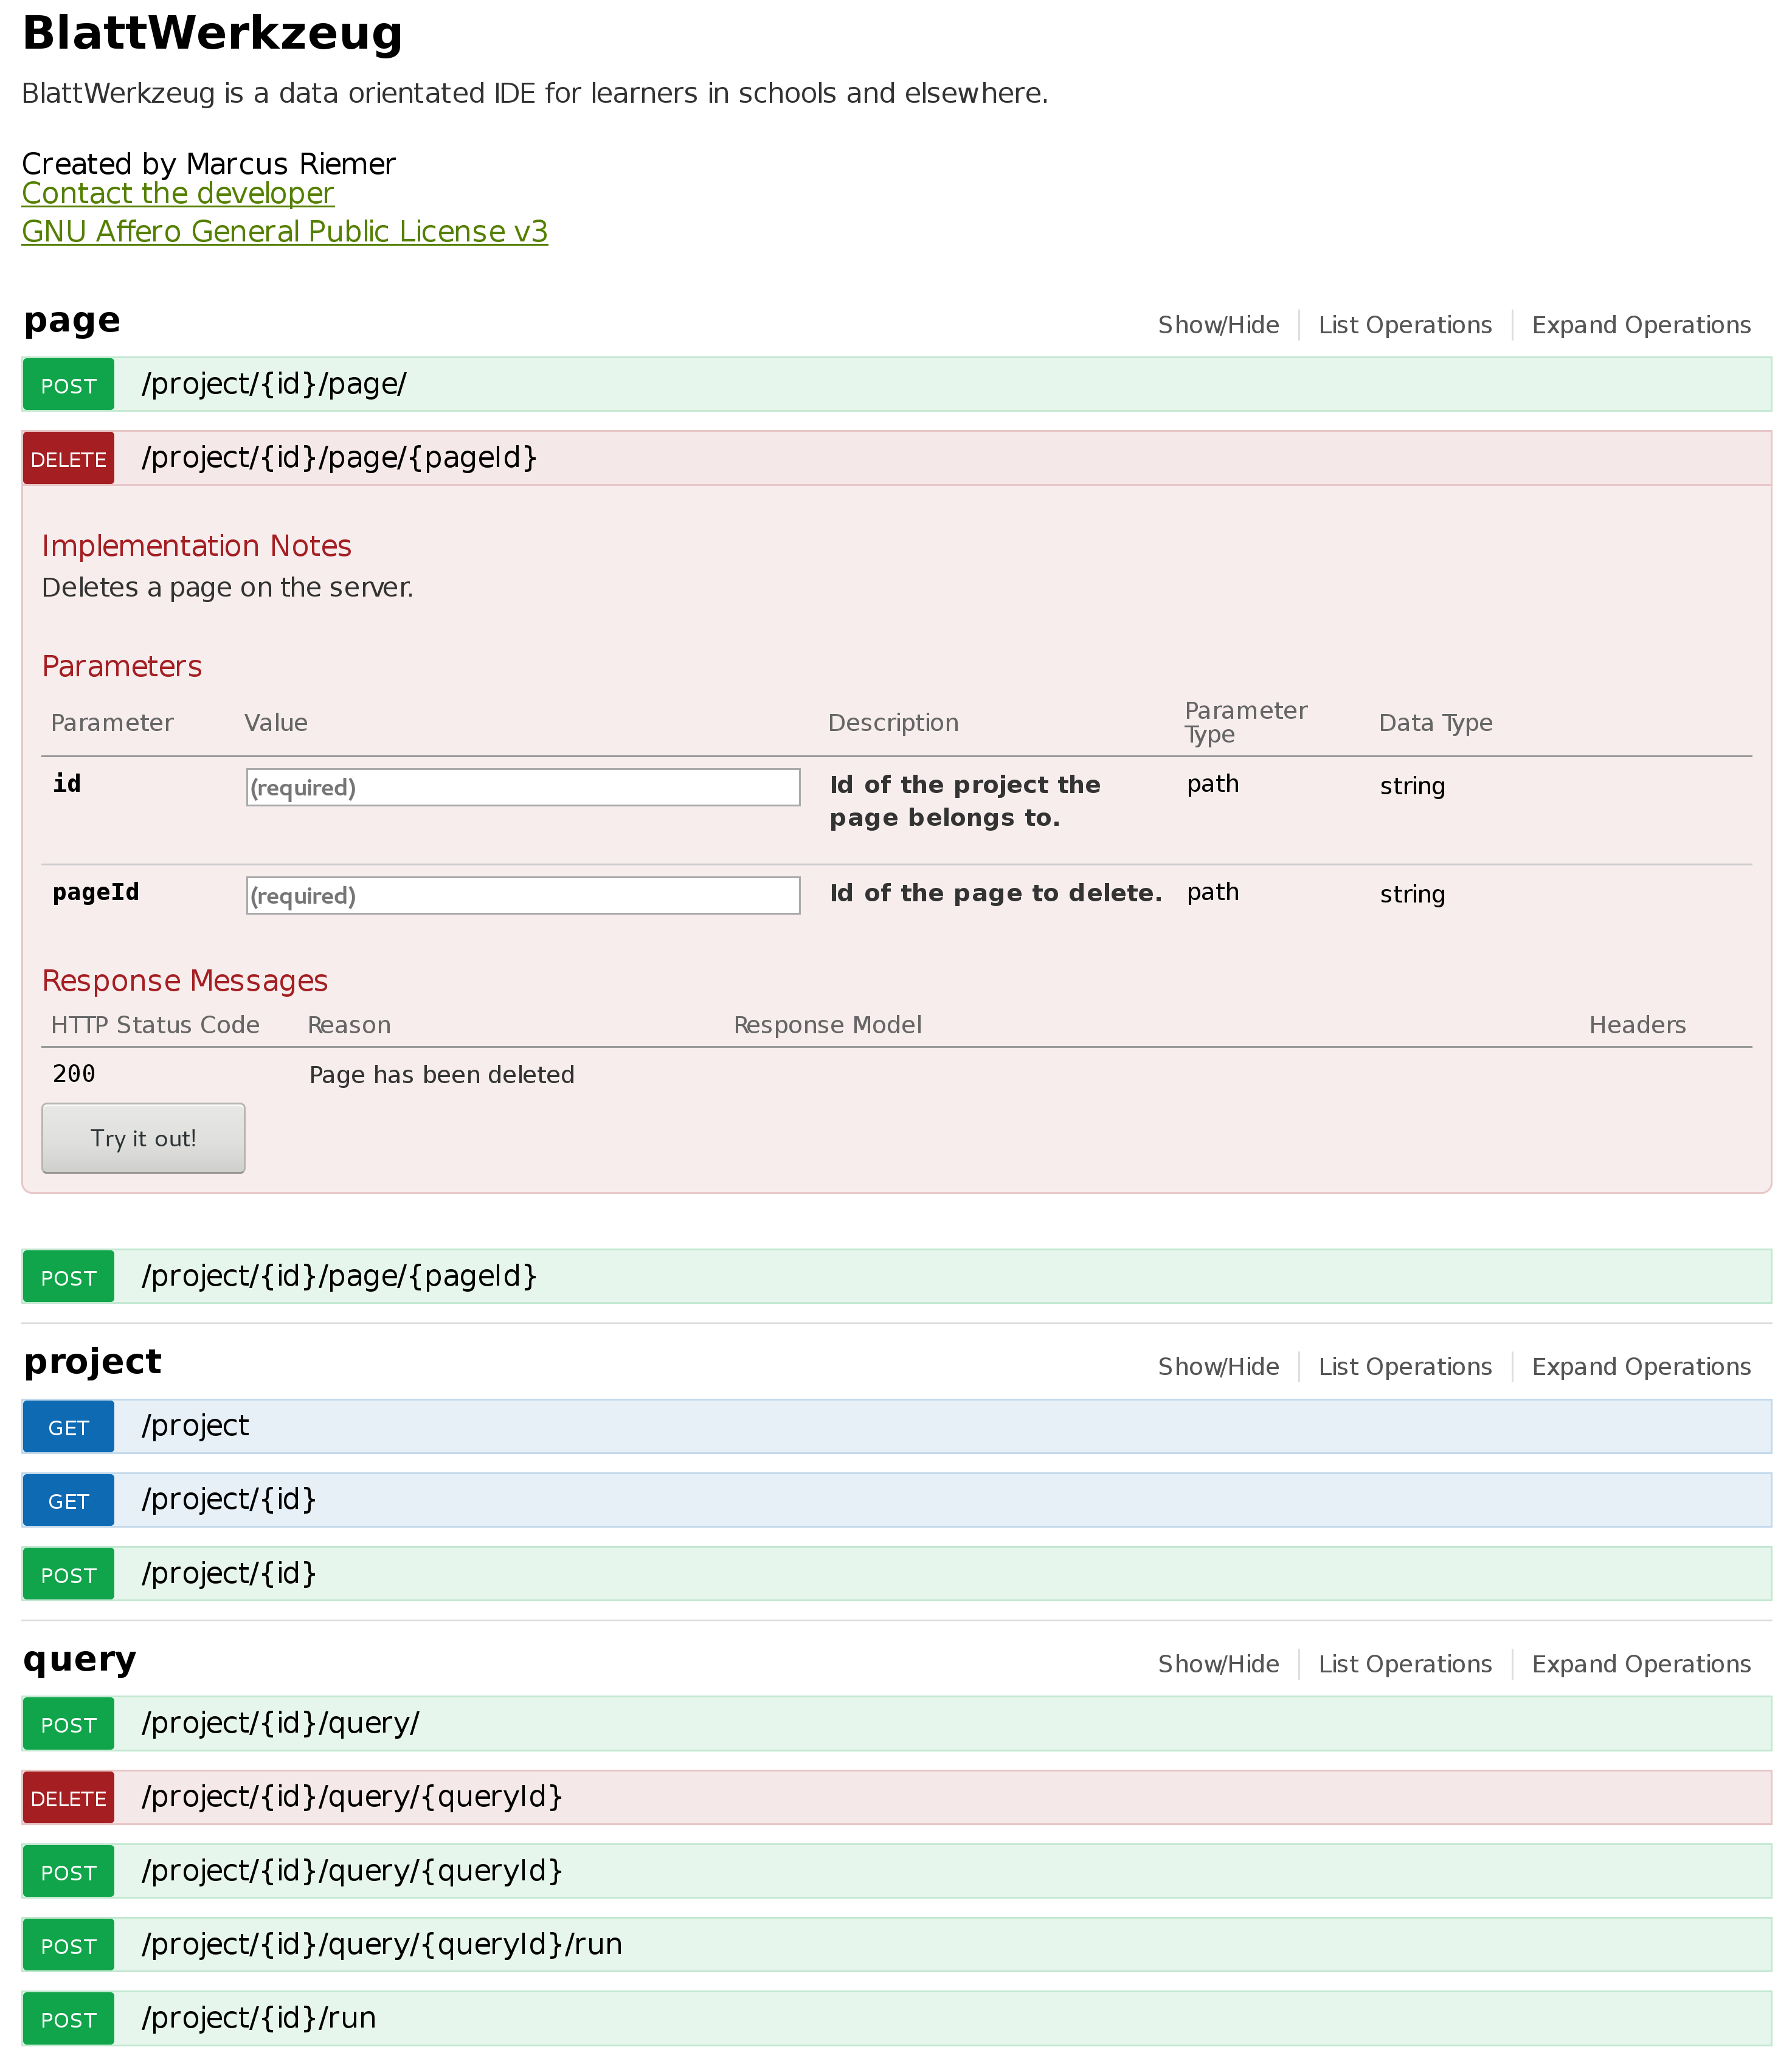
\includegraphics[width=\textwidth]{images/openapi-query-example.png}
  \caption{Generiert aus der Spezfikation: \texttt{API}-Browser für \idename{}}
  \label{fig:openapi-query-example}
\end{figure}

Um die Schnittstelle zwischen diesen beiden Komponenten so transparent wie möglich zu halten, werden diese gemäß der OpenAPI-Spezifikation \cite{open-api} dokumentiert. Dieses offene Format ermöglicht es, auf eine hilfreiche Auswahl an standardisierten Tools aufzubauen. Zum Beispiel können aus der Spezifikation interaktive Testumgebungen für die Server-Schnittstellen erzeugt werden, Abbildung \ref{fig:openapi-query-example} zeigt ein Beispiel dafür\todo{Screenshot zeigt alten Namen}.

Als primäres Interface für die Kompilierung wird ein \texttt{Makefile} genutzt. Dieses prüft, ob auf dem aktuellen System alle nötigen Abhängigkeiten verfügbar sind und stellt sicher, dass Übersetzungsschritte nur ausgeführt werden, wenn sie tatsächlich notwendig sind. Von den technischen Details der unterschiedlichen Programmierumgebungen aufgrund der unterschiedlichen Programmiersprachen kann so außerdem elegant abstrahiert werden: Ein Programmierer kann sich die exakten Aufrufe der unterschiedlichen Paketmanager zwar anschauen, wird im Normallfall aber nur \texttt{make install-deps} aufrufen.

\subsection{Meilensteine}
\label{sec:implementation-roadmap}

Der Editor für Datenbankabfragen versprach im Vergleich zum Seiteneditor das einfachere Teilprojekt zu sein: Die Struktur einer Abfrage ist sehr strikt festgelegt, der Umfang lässt sich gut lokal eingrenzen. Im ersten Schritt wird allerdings nicht der komplette Editor implementiert, sondern zunächst nur das interne Datenmodell für die Abfragen in Form eines abstrakten Syntaxbaumes mitsamt den zugehörigen Tests.

Um den Umfang des Prototypen zu begrenzen, wurde die Implementierungsphase anhand der folgenden funktionalen Meilensteine geplant. Jeder Meileinstein beginnt mit einer kurzen Erläuterung und listet dann die sich daraus ergebenden funktionalen Anforderungen auf.

\begin{description}
\item[Bearbeitung von Projektdaten] \hfill \\
  Schwerpunkt dieses Meilensteins ist die Implementierung grundlegender gemeinsamer Schnittstellen. Diese müssen vom Server als \texttt{HTTP}-Endpunkte angeboten und vom Client angesprochen werden können.
  \begin{itemize}[noitemsep]
  \item Persistierung von Projekten mit Name und Beschreibung
  \item Editor für Projekteigenschaften
  \item Auflistung aller Projekte einer \idename{}-Instanz
  \end{itemize}
  
\item [Anzeige eines Datenbankschemas] \hfill \\
  Neben der funktionalen Anforderung umfasst dieser Meilenstein die Erweiterung des Clients um die typischen Bestandteile der Benutzerschnittstelle einer Entwicklungsumgebung. Serverseitig erfordert dieser Meilenstein zum ersten Mal eine Verbindung mit der Datenbank.
  \begin{itemize}[noitemsep]
  \item Editor zur Anzeige eines Datenbankschemas
  \item Seitenliste mit Übersicht über alle Bestandteile eines Projekts
  \item Toolbar mit Knöpfen, deren Verfügbarkeit vom aktuellen Editor abhängt
  \item Wechsel zwischen verschiedenen Editoren
  \end{itemize}
  
\item [Datenmodell \& Code-Generator für Abfragen] \hfill \\
  Der abstrake Syntaxbaum für Datenbankabfragen in \idename{} sowie dessen Validierung gegen ein Datenbankschema. Dieses Datenmodell soll soweit wie möglich von der Visualisierung entkoppelt werden, damit es sich möglichst einfach testen lässt.
  \begin{itemize}[noitemsep]
  \item Einfache Projektion durch Auswahl von Spalten im \texttt{SELECT}
  \item Kreuzprodukte unterschiedlicher Tabellen im \texttt{FROM}
  \item Einschränkungen der Ergebnismenge mit Ausdrücken im \texttt{WHERE}
  \item Ausdrücke mit binären Operationen zwischen Spalten, Konstanten und benutzerdefinierten Werten
  \item Validierung des Datenmodells mit im Fehlerfall aussagekräftigen Hilfen
  \end{itemize}
  
\item [Editor für Abfragen] \hfill \\
  Implementierung des Drag \& Drop-Editors für SQL-Abfragen. Wesentliche Herausforderung in diesem Schritt wird die Implementierung eines möglichst allgemeingültigen Ansatzes zur Behandlung der Drag \& Drop-Vorgänge sein.
  \begin{itemize}[noitemsep]
  \item Drag \& Drop-Editor für Abfragen
  \item Ausführung von SQL-Abfragen auf dem Server
  \item Clientseitige Anzeige von serverseitigen Ergebnissen
  \end{itemize}
  
\item [Datenmodell \& Code-Generator für darstellende Webseiten] \hfill \\
  Das Datenmodell für Webseiten zur Anzeige der Ergebnisse von \texttt{SELECT}-Abfragen sowie die dazu passenden Testfälle. Auch hier gilt, dass dieses Datenmodell soweit wie möglich von der Darstellungsebene (Angular 2) losgelöst sein soll.
  \begin{itemize}[noitemsep]
  \item Layout mit Zeilen und Spalten
  \item Einfache, textbasierte Elemente wie Absätze und Überschriften
  \item Ausgabe von Abfrageergebnissen in einer Tabelle
  \item Navigation zu projekt-internen und externen Seiten
  \item Übergabe von \texttt{GET}-Parametern an Seiten
  \end{itemize}
  
\item [Rendern von darstellenden Webseiten] \hfill \\
  Um sicherzustellen, dass sich in dem Datenmodell für Seiten aus dem vorigen Meilenstein keine groben Schnitzer befinden, sollen diese nun den Endanwendern zugänglich gemacht werden.
  \begin{itemize}[noitemsep]
  \item Manuelle Erstellung einiger einfach Testprojekte mit Testdaten
  \item Serverseitiges Rendern der verfügbaren Testprojekte
  \end{itemize}
  
\item [Editor für darstellende Webseiten] \hfill \\
  Dieser Schritt profitiert hoffentlich von den Erfahrungen mit dem Drag \& Drop-Editor für SQL. Anders als für den recht offensichtlich "`richtigen"' Ansatz des SQL-Editors hat sich im Rahmen der Analyse für diesen Meilenstein noch keine endgültig favorisierte Darstellung gefunden. Daher ist in diesem Schritt mit mehreren Iterationen bis zur "`richtigen"' Implementierung zu rechnen.
  \begin{itemize}[noitemsep]
  \item Zuordnung von \texttt{SELECT}-Abfragen zu einer Seite
  \item Drag \& Drop-Editor für Seitenelemente
  \item Integrierte Rendervorschau
  \end{itemize}
  
\item[Erweiterung der Seiten um Benutzereingaben] \hfill \\
  Bisher können mit Webseiten nur Informationen präsentiert, aber nicht verändert werden.
  \begin{itemize}[noitemsep]
  \item Einführung des \texttt{<form>}-Elementes in das Datenmodell.
  \item Eingabe von Texten mit dem \texttt{<input>}-Element.
  \item \textit{1 aus n}-Auswahl mit dem \texttt{<select>}-Element.
  \end{itemize}
  
\item [Qualitätssicherung] \hfill \\
  Zu diesem Zeitpunkt sollte ein voll funktionsfähiger Prototyp existieren, der jedoch noch einer rigorosen Qualitätskontrolle unterzogen werden muss. Bisher wurde der Prototyp ausschließlich durch Entwickler bedient, es stellt sich insbesondere die Frage, wie \idename{} auf Bedienfehler oder Inkonsistenzen reagiert.
  \begin{itemize}[noitemsep]
  \item Was passiert mit bestehenden Inhalten, wenn sich das Schema deutlich verändert?
  \item Wie sollten Seiten für Endanwender gerendert werden, wenn diese fehlerhaft sind?
  \end{itemize}
\end{description}

\subsection{Datenbanksystem}
\label{sec:implementation-database-system}

Die Wahl des konkreten Datenbanksystems hat einen unmittelbaren Einfluss auf nahezu alle Bereiche von \idename. Im Einzelnen handelt es sich dabei um die exakte Variante der \texttt{SQL}-Syntax, auf die Rahmenbedingungen für den Betrieb der Entwicklungsumgebung und auch auf die Fortführung der Projekte mit externen Programmen.

Die in der Praxis häufig dominierenden Entscheidungskriterien der Skalierbarkeit, die Unterstützung unterschiedlichster Zugriffsrechte und auch die allgemeine Performance spielen nur eine sehr untergeordnete Rolle. Die zu erwartenden Datenbeständen sollten normalerweise im Bereich nur einiger Megabyte liegen. Die in der Praxis vermutlich einzige relevante Unterscheidung von Zugriffsrechten wäre zwischen allgemeinem lesendem und schreibenden Zugriff, nicht jedoch auf Basis einzelner Datensätze oder komplexer Benutzergruppen.

Für die Wahl des Datenbanksystems werden stattdessen die folgenden Kriterien gewählt und hinsichtlich ihrer Relevanz sortiert:

\begin{description}  
\item[Kostenlose Verfügbarkeit] \hfill \\
  Der Betrieb des Datenbanksystems soll nicht mit Lizenzkosten für Schulen, Lehrkräfte, Lernende oder auch freiwillige Entwickler verbunden sein.
\item[Einfacher Betrieb] \hfill \\
  Zwar ist für den Einsatz von \idename{} aufgrund des Browsers als Client schon die Nutzung eines Servers nötig, das Datenbanksystem sollte den Betrieb aus Sicht von Administratoren der Seite dennoch nicht mehr als unbedingt notwendig verkomplizieren. Eine wesentliche Rolle spielt dabei die Plattformunabhängigkeit: Das Datenbanksystem sollte, wie auch der \idename{}-Server, auf jeder gängigen Betriebssystemfamilie (Windows, MacOS, Linux) lauffähig sein.
\item[Einfache Backups] \hfill \\
  Die gewünschte Exportfunktion für Projekte macht es nötig, den gesamten Datenbestand vergleichsweise einfach exportieren und importieren zu können. Darüber hinaus sollte es auch für Lehrkräfte möglichst einfach sein, mit allen Projekten zu einem anderen \idename{}-Server umzuziehen.
\item[Tools zur Modellierung] \hfill \\
  Da diese Arbeit sich nicht mit der Datenmodellierung befasst, muss das entsprechende Datenbankschema extern erzeugt werden. Von einer guten Unterstützung für Modellierungsvorhaben profitiert dementsprechend indirekt auch \idename.
\item[Externe Tools zur Entwicklung von SQL-Abfragen] \hfill \\
  Sobald ein Entwickler an die Grenzen des \texttt{SQL}-Editors von \idename{} stößt, soll es bei Bedarf so einfach wie möglich sein, die entsprechend komplizierten Abfragen in einem externen Editor zu schreiben und danach in Textform wieder an \idename{} zu übergeben.
\end{description}

Das Kriterium der "`kostenlosen Verfügbarkeit"' ist dankenswerterweise sehr einfach zu erfüllen: Es existiert eine Vielzahl von praktisch eingesetzten quelloffenen Datenbanksystemen. Die Kriterien "`einfacher Betrieb"' und "`einfache Backups"' teilen die denkbaren Systeme recht eindeutig in zwei Lager: Eingebette Datenbanken lassen sich sehr einfach betreiben und sichern. Das starten eines weiteren SQL-Server-Prozesses ist bei dieser Betriebsart nicht nötig, der Im- oder Export des gesamten Datenbestandes erfordert nur das kopieren einer einzigen Datei.

Um den Betrieb folglich so einfach wie möglich zu halten, wurden für \idename{} zunächst eingebettete Datenbanksysteme betrachtet. Aus der Masse an verfügbaren Systemen sticht das SQLite-System jedoch sehr weit hinaus: Der Quelltext ist gemeinfrei, die Anbindung an so ziemlich jede Programmiersprache ist bequem möglich und es existiert eine Fülle von verschiedensten Modellierungsprogrammen für alle Betriebssysteme. Auf eine genauere Analyse der zur Verfügung stehenden Alternativen wurde daher verzichtet.

\subsection{Tests}
\label{sec:implementation-tests}

Die Funktionalität der relativ isolierten und daher gut zu testenden internen Datenmodelle samt den darauf definierten Operationen wird über Unit-Tests sichergestellt. Diese Tests können einfach in jedem Browser ausgeführt werden und eignen sich daher auch, um im Zweifelsfall unterschiedliche Verhaltensweisen verschiedener Browser zu erfassen.

Als technisches Fundament wird für diese Testfälle auf der Jasmine-Bibliothek aufgebaut. Zu prüfende Zusicherungen werden durch Verkettung zweier Funktionen ausgedrückt: \texttt{expect().toEqual()}. Neben \texttt{toEqual()} sind natürlich auch andere Vergleiche wie \texttt{isUndefined()} möglich. Wenn innerhalb eines Testfalls auch nur eine einzige dieser Prüfungen nicht zu \texttt{true} auswertet, wird der Testfall als ingesamt fehlgeschlagen markiert. Im Falle von mehreren gescheiterten Prüfungen werden dabei alle unerwarteten Ergebnisse aufgelistet.

Listing \ref{lst:unit-test-example} illustriert, wie die meisten Unit-Testfälle in \idename{} aufgebaut sind. Jeder Testfall beginnt mit der Definition eines Datenmodells (Zeilen 6 bis 23) und endet mit Zusicherungen, um die korrekte Serialisierung sicherzustellen (Zeile 43). Ganz konkret existiert also in jedem Testfall eine Variable \texttt{model}, welche im Konstruktor der zu testenden Klasse zum Einsatz kommt und in nicht-mutierenden Testfällen als Ergebnis der \texttt{toModel()}-Methode reproduziert werden muss. Für Abfragen muss noch die Generierung der korrekten \texttt{SQL}-Anweisungen geprüft werden, im Beispiel geschieht dies in Zeile 20.

\lstinputlisting[
  language=javascript,
  caption=Unit-Test für eine korrekte \texttt{SELECT}-Abfrage,
  label=lst:unit-test-example,
  float,floatplacement=h,
  numbers=left
]{snippets/unit-test-example.ts}

Die serverseitige Funktionalität wird aktuell ausschließlich über "`end-to-end"'-Tests mit einem speziell instrumentierten Browser geprüft. Für diese Tests ist ein speziell vorbereitetes Testprojekt in einem exakt definierten Zustand Teil des Repositories. Auch diese Testfälle nutzen die von Jasmine bereitgestellten Zusicherungen mit den \texttt{expect()}- und \texttt{toEqual()}-Verkettungen. Listing~\ref{lst:e2e-test-example} zeigt, wie mit einem solchen Test die Funktionaliät des Editors für Projekteinstellungen sichergestellt wird. Mittels der \texttt{browser.get()}-Funktion kann zu einer bestimmten Seite navigiert werden. Um mit den einzelnen Bedienelementen dieser Seite interagieren zu können, müssen diese anhand ihrer \texttt{ID} oder anderer eindeutiger Merkmalen zugreifbar sein (Zeilen 6, 8 und 14 des Listing~\ref{lst:e2e-test-example}). Dann können für solche Elemente Tastatureingaben simuliert oder der Inhalt verglichen werden. Bestimmendes Merkmal dieser Tests zum Speichern ist, dass sie die initial geladene Seite nach dem Speichervorgang erneut aufrufen. Nur wenn die zuvor gesetzten Werte auch nach diesem Ladevorgang noch vorhanden sind, kann von der korrekten Funktionsweise des Servers ausgegangen werden.

\lstinputlisting[
  language=javascript,
  caption=End-to-end Test für den Speichervorgang eines Projektes,
  label=lst:e2e-test-example,
  float,floatplacement=h,
  numbers=left
  ]{snippets/e2e-test-example.ts}

Die Dateien mit den Tests liegen im Dateisystem immer "`neben"' ihren Implementierungen, der Dateiname wird allerdings um das Suffix \texttt{spec} wie "`specification"' oder \texttt{e2e} wie "`end-to-end"' ergänzt. Das Beispiel in Listing  \ref{lst:unit-test-example} wurde der Datei \texttt{select.spec.ts} entnommen, der Code für die zu testende Funktionalität findet sich folglich in \texttt{select.ts}.

\subsection{Datenmodell}

Die grundsätzliche Struktur eines \idename-Projektes wird in Diagramm \ref{uml:class-diagram-core-entities} ersichtlich. Diese Darstellung visualisert nicht die konkrete Implementierung des Servers oder des Clients, sondern illustriert die grundlegenden beteiligten Datenstrukturen. Jede dieser Entitäten, also sowohl Projekte als auch ihre Ressourcen, enthält eine eigene Versionsangabe. Dadurch kann auf jede Veränderung an dieser Struktur explizit eingegangen werden (\fullref{sec:implementation-migration}). Aktuell laden sowohl Server als auch Client nur Ressourcen, deren Version exakt passt.

Jede Ressource (\texttt{ProjectResource}) verfügt über eine interne ID sowie einen sprechenden Namen. In der aktuellen Version von \idename{} handelt es sich bei dieser ID um eine \texttt{GUID}, sie sollte also weltweit einzigartig sein. Theoretisch wäre es dadurch denkbar, diese Ressourcen auch zwischen Projekten zu kopieren oder zu teilen. Intern werden Referenzen auf Ressourcen immer anhand der ID vorgenommen. Eine Umbenennung von Ressourcen durch den Benutzer hat daher keine Auswirkungen auf etwaige Referenzen an anderer Stelle.

Die Methode \texttt{ProjectResource.toModel()} wird genutzt, um aus dem spezifischen Res\-sour\-cen-Objekt eine rein beschreibende Datenstruktur zu erzeugen. Diese Beschreibung ist selbstverständlich abhängig vom Typ der jeweiligen Ressource und kommt auch in dessen Konstruktor zum Einsatz. Tiefe Kopien von Ressourcen können daher über diese Se\-ria\-lisierungs- und Deserialisierungsschritte vorgenommen werden.

\begin{diagram}[p]
  \begin{tikzpicture}
    \begin{interface}[text width=7cm]{ApiVersionable}{-4, 0}
      \attribute{apiVersion : string}
    \end{interface}
    
    \begin{class}[text width=7cm]{Project}{-8, -4}
      \implement{ApiVersionable}
      
      \attribute{id : string}
      \attribute{name : string}
      \attribute{description : string}
      \attribute{indexPageId : string}
    \end{class}

    \begin{abstractclass}[text width=7cm]{ProjectResource}{0, -6}
      \implement{ApiVersionable}

      \operation[0]{toModel() : ProjectResource}
      
      \attribute{id : string}
      \attribute{name : string}
    \end{abstractclass}

    \begin{class}[text width=7cm]{Page}{0, -10}      
      \attribute{body: BodyNode}
      \attribute{referencedQueries: QueryReference[]}
      \attribute{parameters: PageParameter[]}
    \end{class}

    \begin{class}[text width=7cm]{Query}{0, -14}
      \attribute{select : Select}
      \attribute{delete : Delete}
      \attribute{insert : Insert}
      \attribute{update : Update}
      \attribute{from   : From}
      \attribute{where  : Where}
    \end{class}

    % query and page implement projectresource
    \draw[->] (Query.east) -- ++ (1,0) -- ($(ProjectResource.east)+(1,0)$) -- (ProjectResource.east);
    \draw[-] (Page.east) -- ++ (1,0);

    % each resource has a reference to the project
    \draw[] (ProjectResource.north)  |- (Project.east);
    \node[xshift=0.3cm, yshift=0.3cm] at (ProjectResource.north) {n};
    \node[xshift=0.3cm, yshift=0.3cm] at (Project.east) {1};
    
    % a project has pages ...
    \draw[] (Page.west)  -| (Project.south);
    \node[xshift=0.3cm, yshift=-0.5cm] at (Project.south) {1};
    \node[xshift=-0.5cm, yshift=0.3cm] at (Query.west) {0..n};
    \node[xshift=-2.5cm, yshift=0.3cm] at (Query.west) {Queries};

    % ... and queries.
    \draw[] (Query.west) -| (Project.south);
    \node[xshift=-0.5cm, yshift=0.3cm] at (Page.west) {0..n};
    \node[xshift=-2.5cm, yshift=0.3cm] at (Page.west) {Pages};
  \end{tikzpicture}

  \caption{Abstrakte Übersicht über die Ressourcen eines Projektes}
  \label{uml:class-diagram-core-entities}
\end{diagram}

\subsubsection{Serverseitige Persistenz}
\label{sec:implementation-persistence}

Grundsätzlich sollte die serverseitig persistierte Repräsentation einer Ressource identisch mit dem Übertragungsformat sein. Dieses Vorgehen spart durch die Einsparung eines Transformationsvorganges potenziell Zeit, vor allem erleichtert es aber die serverseitige Implementierung. Bei der folgenden Betrachtung von möglichen Optionen zur Speicherung der Daten wird also grundsätzlich von \texttt{JSON}-Dokumenten ausgegangen. Bei der Auslieferung durch den Server können diese dann möglicherweise sogar unverändert weitergereicht werden. Um die Persistierung vorzunehmen, kommen im Wesentlichen zwei Speichermethoden in Frage: Entweder werden Datensätze direkt als Datei im Dateisystem abgelegt oder in einer dokumentenorientierten Datenbank gespeichert.

Bei einer Speicherung im Dateisystem wäre der rein lesende Zugriff auf \idename-Datensätze sogar mit einem einfachen Webserver für statische Dateien möglich. Um ein Projekt zu Testzwecken anzusehen oder zu editieren, reicht ein normaler Texteditor. Neue Projekte können einfach per Copy \& Paste im Dateisystem angelegt werden. Perspektivisch wäre es relativ einfach möglich, ein Projekt mit gängigen Versionsverwaltungsprogrammen wie git oder mercurial zu versionieren. Diese Implementierung besticht also vor allem durch ihre Einfachheit in Bezug auf die zum Zugriff notwendigen Programme.

Die Speicherung in dokumentenorientierten Datenbanken wie MongoDB oder in einem Key/Value-Store wie redis macht den Zugriff auf die persistierten Daten abhängig von einem externen Serverprozess. Der universelle Zugriff über das Dateisystem weicht einem speziellen Programm zur Navigation innerhalb der jeweiligen Datenbank. Mit dieser Komplexität erkauft man auf der anderen Seite eine wesentlich größere Flexibilät in Bezug auf horizontale Skalierung: Sollte es jemals notwendig werden, den Server auf mehr als einem Rechner zu betreiben, existiert dafür dann schon eine hilfreiche Basis.

Letzten Endes fiel die Entscheidung auf das Dateisystem. Die Gründe ähneln jenen, wie sie schon bei der Wahl von \texttt{SQLite} aufgezählt wurden (\fullref{sec:implementation-database-system}): Backups des Dateisystems sind trivial, externe Programme für diesen Zweck sind zahlreich vertreten. Sollte eine komplizierte Lösung notwendig werden, kann man diese immer noch implementieren, sobald sie tatsächlich benötigt wird.

Technisch gesehen ist ein Projekt folglich eine Sammlung von Dateien in einer festgelegten Ordnerstruktur. Abbildung~\ref{fig:project-disk-structure} zeigt ein beispielhaftes Projekt mit jeweils einer Datenbank, Abfrage und Webseite.

\begin{figure}[h!]
  \dirtree{%
    .1 example-project/.
    .2 databases/.
    .3 default.sqlite.
    .2 queries/.
    .3 0c396a9a-1947-4c2b-a5fb-195df2b91b84.json.
    .3 0c396a9a-1947-4c2b-a5fb-195df2b91b84.sql.
    .2 pages/.
    .3 0a436465-b074-46a4-ac12-b091a77c9d6b.json.
    .3 0a436465-b074-46a4-ac12-b091a77c9d6b.liquid.
    .2 config.yaml.
  }
  \caption{Dateistruktur eines Projekts}
  \label{fig:project-disk-structure}
\end{figure}

Dabei werden Seiten und Abfragen in zwei Versionen gespeichert: Einmal das \texttt{JSON}-serialisierte Datenmodell und eine jeweils "`kompilierte"' Version in Form von \texttt{SQL}- oder Liquid-Code.

\subsubsection{Projekt}
\label{sec:data-model-project}

Die vornehmlichen Eigenschaften eines Projektes sind die darin enthaltenen Abfragen und Webseiten, darüber hinaus werden in den Projekteinstellungen aber noch einige andere Einstellungen festgehalten:

\begin{description}[noitemsep]
\item[Name, Beschreibung \& Bild] \hfill \\
  Von Entwicklern frei wählbare Elemente, mit denen das Projekt einem Endanwender kurz und knapp beschrieben wird. Der Prototyp erlaubt zum aktuellen Zeitpunkt noch nicht den Upload von Bildern, Endanwendern werden die Bilder in der Projektübersicht aber dennoch angezeigt.\todo{Screenshot}
\item[Aktivierte Datenbank] \hfill \\
  Ein Entwickler kann in einem Projekt zwischen mehreren "`Evolutionsstufen"' oder Sicherheitskopien einer Datenbank auswählen. Für einen Endanwender ist diese Unterscheidung allerdings nicht von Relevanz: Er erwartet nicht beim erstmaligen Besuch einer Seite zunächst eine Datenbank auswählen zu müssen. Daher legt der Entwickler in dieser Einstellung fest, welche Datenbank zum Rendern verwendet werden soll.
\item[Startseite] \hfill \\
  Sobald in einem Projekt mehr als eine Webseite verfügbar ist, muss eine dieser Seiten als Startseite festgelegt werden.
\item[Benutzerdatenbank] \hfill \\
  Die in Kapitel \fullref{sec:concept-access-control} beschriebenen Zugriffskontrollen bedürfen einer rudimentären Benutzerdatenbank. Aktuell wird diese als Teil des Projekts gespeichert, die Passwörter werden dabei selbstverständlich verschlüsselt.
\item[Routendefinitionen] \hfill \\
  Der aktuelle Stand der Implementierung erstellt für jede existierende Seite implizit eine Route, die einfach dem Namen der Seite entspricht. Eine Seite mit dem Namen "`impressum"' ist folglich unter der \texttt{URL} "`\texttt{http://projekt.server.tld/impressum}"' erreichbar. 
\end{description}

\subsubsection{Abfrage}
\label{sec:data-model-query}

Das Datenmodell für Abfragen teilt sich in zwei wesentliche Bereiche auf: Einerseits die Repräsentation der \texttt{SQL}-Komponenten wie \texttt{SELECT}, \texttt{FROM}, ... und andererseits die in fast allen Komponenten denkbaren Ausdrücke.

\subsubsection{Seite}

\subsection{Client}

\subsubsection{Existierende Implementierungen von Drag \& Drop-Editoren}

Die Drag \& Drop-Editoren sind allesamt von Grund auf getätigte Eigenentwicklungen, welche direkt auf der \texttt{HTML5}-Spezifikation aufsetzen. Im Rahmen des schon vorgestellten App Inventor (\fullref{sec:related-app-inventor}) wurde von Google allerdings ebenfalls eine quelloffene Bibliothek für Drag \& Drop-Editoren namens "`Blockly"' entwickelt\footnote{\url{https://developers.google.com/blockly/}}. Warum wurde für \idename{} also eine Eigenentwicklung forciert?

Um Blockly zu evaluieren ist ein sehr kleiner Prototyp zur Bearbeitung von \texttt{SQL}-Abfragen entwickelt worden (Abbildung~\ref{fig:blockly-eval-sql}). Dabei hat sich kein schlagender Grund gegen Blockly gefunden, stattdesen aber eine recht lange Liste von technischen und inhaltlichen Aspekten, die nicht so recht zu \idename{} passen.

\begin{figure}[h]
  \centering \includegraphics[width=0.6\textwidth]{images/blockly/first-steps}
  \caption{Grundzüge eines \texttt{SQL}-Editors mit Blockly}
  \label{fig:blockly-eval-sql}
\end{figure}

\begin{itemize}[noitemsep]
\item Es handelt sich bei Blockly um eine Bibliothek für imperative Programmiersprachen, inklusive Code-Generatoren für zum Beispiel Python, Javascript, Lua, ... Eine Unterstützung von \texttt{HTML} oder \texttt{SQL} ist nicht vorgesehen und müsste selber implementiert werden.
  
\item Code-Elemente werden in Blockly standardmäßig frei auf einer zweidimensionalen Zeichenfläche platziert. Um innerhalb eines Kontextes auf Ereignisse zu reagieren ist dieser Ansatz sinnvoll. Für \idename{} gilt jedoch, dass jedes zu bearbeitende Element feste Einstiegspunkte hat: \texttt{SELECT} und \texttt{FROM} bei lesenden \texttt{SQL}-Abfragen, \texttt{<body>} und möglicherweise \texttt{<head>} für Webseiten. Die mehrfache Verwendung dieser Wurzelelemente ist inhaltlich nicht sinnvoll, eine freie Platzierung bietet keinen signifikanten Mehrwert.

\item Das von Blockly verwendete Datenmodell enthält Details zur grafischen Darstellung und eignet sich nicht gut zur abstrakten Repräsentation von \texttt{HTML} oder \texttt{SQL}. Dieses Format kommt daher im Hinblick auf andere Arten von Editoren, zum Beispiel einem \texttt{WYSIWYG}-Editor für Oberflächen, nicht als exklusives Format in Frage. Dementsprechend müsste immer zwischen den eigentlichen \idename{}-Formaten und Blockly hin und zurück übersetzt werden.
  
\item Blockly versteht sich nicht nur als Oberflächenbibliothek, sondern auch als Code-Generator. Dieser Aspekt wird in \idename{} aber losgelöst von der grafischen Repräsentationen durch einzelne Editoren betrachtet. Diese Funktionalität von Blockly müsste daher aktiv ignoriert werden, da einzelne Schnittstellen das Vorhandensein entsprechender Funktionalität voraussetzen.
  
\item Blockly geht zunächst von einem statisch großen Zeichenbereich aus, um diesen in der Größe zu verändern muss auf globale \texttt{onResize}-Ereignisse reagiert werden. \idename{} kommt hingegen mit ausschließlich per \texttt{CSS} gehandhabten Größenangeben aus, was im Endeffekt permanent korrekte Größenverhältnisse garantiert. Die offizielle "`Resizeable Blockly"'-Demo\footnote{\url{https://blockly-demo.appspot.com/static/demos/resizable/overlay.html}} lässt sich hingegen durch Nutzung der Entwicklerfunktionen zur Bildschirmgrößen-Vorschau in Chrome und Firefox aus dem Tritt bringen.

\end{itemize}

Da \idename{} zumindest perspektivisch die Verwendung von unterschiedlichen Editoren für identische Inhalte vorsieht, ist Blockly damit keinesfalls endgültig aus der Welt. Spätestens bei einer hypothetischen Integration von "`echten"' Programmiersprachen in \idename{} wird eine Integration wieder zur Diskussion stehen.

\subsection{Server}

\subsubsection{Nutzung von Subdomains}

\idename{}-Projekte werden unter jeweils eigenen Subdomains zur Verfügung gestellt. Das erhöht zwar die Anforderungen an die technische Infrastruktur, geht jedoch mit einer Reihe von Vorteilen einher. Die online bereitgestellte Fassung des Protoypen geht in Bezug auf die zur Verfügung stehenden Subdomains noch einen Schritt weiter: Die Domain für die Entwicklungsumgebung (\href{http://blattwerkzeug.de}{\texttt{blattwerkzeug.de}}) unterscheidet sich von jener für die Projekte (zum Beispiel \href{http://cyoa.blattzeug.de}{\texttt{cyoa.blattzeug.de}}).

Der hauptsächliche Grund für dieses Vorgehen ist die im Internet weitestgehend gültig Annahme, dass auf jeder (Sub-)Domain nur ein logischer Internetauftritt hinterlegt ist. Das sich hinter einer \texttt{URL} wie \texttt{blatt\-werk\-zeug.de\-/project\-/pokemongo} eine völlig andere Seite als hinter \texttt{blatt\-werk\-zeug.de\-/project\-/cyoa} verbirgt ist zwar in keinster Weise verboten, aber zumindest ungewöhnlich.

Praktisch werden Subdomains von vielen Suchmaschinen, sonstigen Angeboten im Internet und auch innerhalb der technischen Standards, anders behandelt, als wenn die gleichen Inhalte als untergeordnete \texttt{URL} einer anderen Seite existierten. Das beginnt schon bei entscheidenden technischen Details: So können zum Beispiel Zertifikate für \texttt{SSL}-Verbindungen nur für Domains, nicht aber für Teile einer \texttt{URL} ausgestellt werden. Und Webseiten werden im Falle von unerwünschten Inhalten, zum Beispiel Phishing-Angriffen, üblicherweise auf Basis von Domainnamen gesperrt.

Darüber hinaus kann unter dieser Voraussetzung jede Webseite davon ausgehen, dass die gesamte Routing-Hierarchie nur ihr gehört. Die Subdomains erlauben also die Nutzung von absoluten Pfadangaben. Insbesondere um Bilder, \texttt{CSS}-Dateien oder JavaScript-Bibliotheken zu verlinken, ist das eine hilfreiche Garantie, welche viele unpraktische Probleme vermeidet.

\subsection{Unerwartete Hindernisse}
\label{sec:unexpected-problems}

\subsubsection{Instabile API von Angular 2}

\subsubsection{Fehlerhafte Codegenerierung des Typescript-Compilers}

Der verwendete Typescript-Compiler hat zum Zeitpunkt der Anfertigung dieser Arbeit einen bekannten Bug in der Codegenerierung \cite{ts-compiler-class-order-bug}, um den wiederholt herumgearbeitet werden musste. Konkret äussert sich dieser Fehler, wenn die Definition der Oberklasse einer sich davon ableitenden Klasse erst im Nachhinein erfolgt (Listing \ref{lst:ts:class-order-bug}). In diesem Fall kommt es zu keiner Warnung durch den Compiler, sondern zu einem Laufzeitfehler im kompilierten Javascript-Code.

\lstinputlisting[language=JavaScript,caption=Falsche Reihenfolge der Klassendefinition, label=lst:ts:class-order-bug]{snippets/class-inheritance-order-bug.ts}

\subsection{Administration}
\label{sec:implementation-administration}

Momentan aufgrund von Zeitmangel nur in Form der Kommandozeilenschnittstelle.

\subsubsection{Schema-Migrationen}
\label{sec:implementation-migration}

%%% Local Variables:
%%% mode: latex
%%% TeX-master: "thesis"
%%% End:
